\documentclass{article}
\usepackage{graphicx}
\usepackage{amsmath}
\usepackage{hyperref}

\begin{document}

\title{Solutions to hw4 homework on Convex Optimization https://web.stanford.edu/class/ee364a/homework.html}
\author{Andrei Keino}
\maketitle
% from 
% https://www.studocu.com/en-us/document/stanford-university/convex-optimization-i/assignments/2020-hw4sol-hw4/7518536/view
% 5.1, 5.3, 5.12, A3.3, A3.10, A3.32 
\section*{5.1}
A simple example. Consider the optimization problem 
\begin{align*}
&minimize \qquad x^2 + 1 \\
&subject \; to  \qquad (x - 2)(x - 4) \leq 0
\end{align*} 
with variable $x \in R$\\

(a) Analysis of primal problem. Give the feasible set, the optimal value, and the optimal solution.\\

(b) Lagrangian and dual function. Plot the objective
$x^2 + 1$ versus $x$. On the same plot,
show the feasible set, optimal point and value, and plot the Lagrangian $L(x, \lambda)$ versus $x$ for a few positive values of $\lambda.$ Verify the lower bound property $(p^* \leq \inf_x L(x, \lambda) \;for\; \lambda \geq 0 ).$ Derive and sketch the Lagrange dual function $g$. \\

(c) Lagrange dual problem. State the dual problem, and verify that it is a concave maximization problem. Find the dual optimal value and dual optimal solution $\lambda ^*$. Does strong duality hold? \\

(d) Sensitivity analysis. Let $p^*(u)$ denote the optimal value of the problem 
\begin{align*}
&minimize \qquad x^2 + 1 \\
&subject \; to  \qquad (x - 2)(x - 4) \leq u
\end{align*} 
as a function of the parameter $u.$ Plot $p^*(u).$ 
Verify that $dp^*(0) / du = - \lambda^*.$ \\

Solution: \\

(a)\\

The feasible set is $x \in [2, 4] $. The optimal solution is 
$x^* = 2$, the optimal value is $p^* = 5.$ \\

(b)\\
% https://www.latex-tutorial.com/tutorials/figures/
\begin{figure}[h!]
	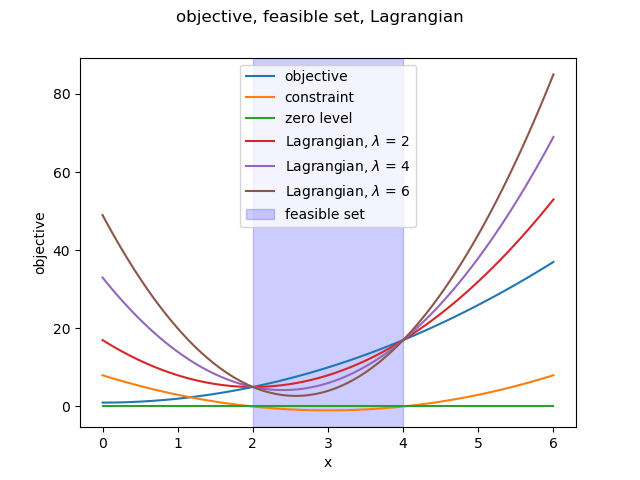
\includegraphics[width=\linewidth]{5_1_b_1.png}
	\caption{objective, feasible set, lagrangian for this problem.}
	\label{fig:5_1_b_1}
\end{figure}

It's easy to see from the Figure 1, that the Lagrangian values on the feasible set are less or equal than the objective values on the feasible set, 
i. e. \\ 
$(p^* \geq \inf_x L(x, \lambda) \;for\; \lambda \geq 0 ).$ \\

(c)\\
The dual objective function for this problem can be found solving the constrained equation for the Lagrangian: \\

\begin{align*}
&g(\lambda) = inf_{x} (x^2 + 1 + \lambda (x - 2)(x - 4))\\
&subject \; to  \qquad \lambda \geq 0
\end{align*} 

The Lagrangian reaches its minimum at the point 
$\tilde x = \frac{3 \lambda}{\lambda + 1}.$
Then the dual objective itself is: \\
$$g(\lambda) = - \lambda + 10 - \frac{9}{(\lambda + 1)}$$ \\
The second derivative of the dual function is:\\
$$g^{''}(\lambda) = - 18 / (\lambda + 1)^3$$
which is obviously less than zero for $\lambda \geq 0,$ i.e. the dual function is concave for $\lambda \geq 0.$


\begin{figure}[h!]
	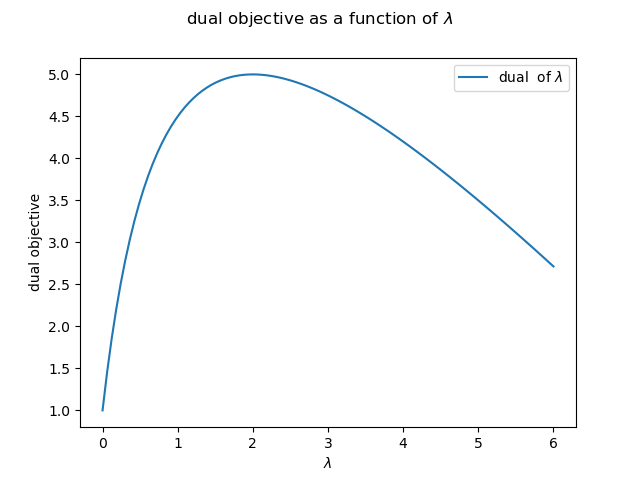
\includegraphics[width=\linewidth]{5_1_b_2.png}
	\caption{Dual objective for this problem.}
	\label{fig:5_1_b_2}
\end{figure}

The dual optimal value $\lambda ^*$ can be found solving the dual problem for the $g(\lambda):$
\begin{align*}
&maximize \qquad g(\lambda) \\
&subject \; to  \qquad \lambda \geq 0
\end{align*} 

or 
\begin{align*}
&d g(\lambda) / {d \lambda} = 0 \\
&subject \; to  \qquad \lambda \geq 0
\end{align*} 

Solving the equation we found $\lambda ^* = 2;$ optimal value of $g$ (i.e. $sup_\lambda \{g(\lambda)\}$) $g^* = 5.$
We can see that $p^* = 5 = g^*,$ i. e. strong duality holds.\\

(d) \\

Solving the constraints equation $(x - 2)(x - 4) = u$ we get:\\
$x_{1, 2} = 3 \pm \sqrt{1 + u}, \; u \geq 1.$ Then \\

\begin{equation}
p^*(u) =
\begin{cases}
	\text{not exists},			& \text{if } u < -1 \\
	u - 6 \sqrt{1 + u} + 11, 	& \text{if } - 1 \leq u \leq 8  \\
	1, 							& \text{if } u > 8
\end{cases}       
\end{equation}

\begin{figure}[h!]
	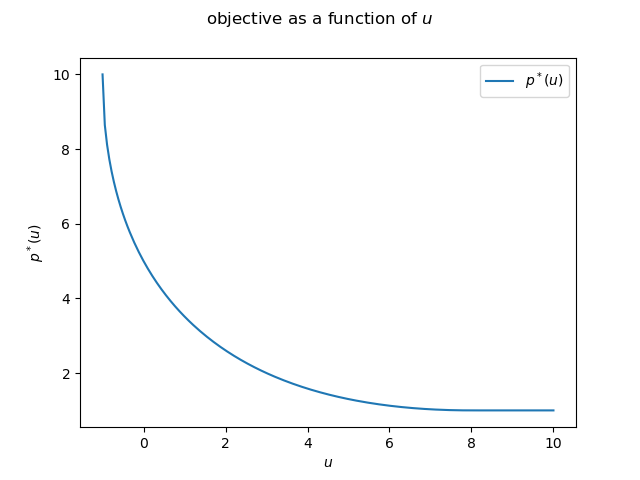
\includegraphics[width=\linewidth]{5_1_3.png}
	\caption{Graph of $p^*(u)$ for this problem.}
	\label{fig:5_1_3}
\end{figure}

And finally:
$$dp^*(u) / du = 1 - \frac{3}{\sqrt{1 + u}}$$
Then $dp^*(0) / du = -2 = - \lambda^*$

\section*{5.3}

Problems with one inequality constraint. Express the dual problem of 
\begin{align*}
&\text{minimize }  c^Tx \\
&\text{subject to }  f(x) \leq 0
\end{align*} 
with $c \neq 0$ in terms of the conjugate $f^*.$ Explain why the problem you give is convex. We do not assume $f$ is convex. \\

Solution: \\
The dual problem of the task is:
\begin{align*}
&\text{maximize }  \inf_x (c^Tx + \lambda f(x)) \\
&\text{subject to }  \lambda \geq 0
\end{align*} 
The definition of the conjugate function is:
$$ f^*(y) = \sup_x (y^T x - f(x)) = - \inf_x(f(x) - y^Tx)$$\\
i.e. the dual problem can be reformulated as:

\begin{align*}
&\text{maximize }  F(c, \lambda) \\
&\text{subject to }  \lambda \geq 0
\end{align*} 
where $F(c, \lambda) = - \lambda f^*(-c/\lambda), $
where $f^*$ is the conjugate function of $f,$ and it is always convex.  $F(c, \lambda)$ is the concave function, as it is the negative perspective of the convex function $f^*$.

\section*{5.12}
Analytic centering. Derive a dual problem for 
$$\text{minimize } - \sum_{i = 1}^{m} log(b_i - a_i^T x)$$
with domain 
$\{x\; | \;  a_i^T x \leq b_i, \; i = 1, ..., m\}.$ First introduce new variables $y_i$ and equality constraints $y_i = b_i - a_i^T x.$ (The solution of this problem is called the analytic center of the linear inequalities $a_i^T x \leq b_i, \; i = 1, ..., m\}.$ 
Analytic centers have geometric applications and play an
important role in barrier methods. \\

Solution:

This problem is equivalent to:
\begin{align*}
\text{minimize } \qquad & - \sum_{i = 1}^{m} log(y_i) \\
\text{subject to } \qquad &y + A x - b = 0 \\
\end{align*}
where the matrix $A$ composed from the rows $a_i^T,$ the $i$ - th row of $A$ is $a_i^T$\\
Then the Lagrangian is\\
$$
L(x, y, \nu) = - \sum_{i = 1}^{m} log(y_i) + 
\nu^T(y + A x - b)
$$
The dual function is
$$
g(v) = \inf_{x, y}( - \sum_{i = 1}^{m} log(y_i) + 
\nu^T(y + A x - b))
$$

The term $\nu^TAx$ is unbounded below as 
$x \rightarrow \infty,$ so \\

\begin{equation*}
g(\nu) =
\begin{cases}
\sum_{i = 1}^{m} log(y_i) + m - \nu^T b , 	
& A \nu = 0, \; \nu_i \geq 0  \\
- \infty, 					& A \nu \neq 0 
\end{cases}       
\end{equation*}

and the dual problem is:

\begin{align*}
\text{maximize } \qquad 
& \sum_{i = 1}^{m} log(\nu_i) + m - \nu^T b \\
\text{subject to } \qquad & A \nu = 0
\end{align*}

\section*{A3.3}
Reformulating constraints in CVX*. Each of the following CVX code fragments describes a convex
constraint on the scalar variables x, y, and z, but violates the CVX rule set, and so is invalid. Briely explain why each fragment is invalid. Then, rewrite each one in an equivalent form that conforms to the CVX rule set. In your reformulations, you can use linear equality and inequality constraints, and inequalities constructed using CVX functions. You can also introduce additional variables, or use LMIs. Be sure to explain (briefly) why your reformulation is equivalent to the original constraint, if it is not obvious.
Check your reformulations by creating a small problem that includes these constraints, and solving it using CVX. Your test problem doesn't have to be feasible; it's enough to verify that CVX processes your constraints without error.
Remark. This looks like a problem about `how to use CVX software', or `tricks for using CVX'.
But it really checks whether you understand the various composition rules, convex analysis, and
constraint reformulation rules.\\ \\
(a) norm([x + 2*y, x - y]) == 0 \\
(b) square(square(x + y)) \textless= x - y\\
(c) 1/x + 1/y \textless= 1; x \textgreater = 0; y \textgreater = 0\\
(d) norm([max(x,1), max(y,2)]) \textless= 3*x + y\\
(e) x*y \textgreater= 1; x \textgreater= 0; 
y \textgreater= 0\\
(f) (x + y)\^{}2/sqrt(y) \textless= x - y + 5\\
(g) x\^{}3 + y\^{}3 <= 1; x \textgreater= 0; y \textgreater= 0\\
(h) x + z <= 1 + sqrt(x*y - z\^{}2); x \textgreater= 0; y \textgreater= 0\\

Solution: \\

(a)  norm([x + 2*y, x - y]) == 0 \\

This constraint is invalid because {\bf Three types of constraints may be specified in disciplined convex programs:\\
}

\begin{itemize}
	\item An equality constraint, constructed using ==, where both sides are affine.
	\item A less-than inequality constraint, using \textless=, where the left side is convex and the right side is concave.
	\item A greater-than inequality constraint, using \textgreater=, where the left side is concave and the right side is convex.
\end{itemize}

\url{http://web.cvxr.com/cvx/doc/dcp.html#constraints}

Expression in (a) violates the first rule - both sides must be affine. As the given norm could be zero only if $(x, y) = (0, 0)$, the workaround:

\begin{verbatim}
subject to
	x == 0;
	y == 0;
\end{verbatim}

The test script: \\
\begin{verbatim}
cvx_begin
variable x;
variable y;
minimize(norm(x + y + 1));
subject to
x == 0;
y == 0;
cvx_end

fprintf('status:'); 
disp(cvx_status);

fprintf('optimal value:'); 
disp(cvx_optval )

fprintf('optimal x:\n'); 
disp(x)

fprintf('optimal y:\n'); 
disp(y)
\end{verbatim}


(b) square(square(x + y)) \textless= x - y\\
this code violates the one of the composition ruleset:\\
\url{http://web.cvxr.com/cvx/doc/dcp.html#expression-rules}\\
{\bf
If the function is neither nondecreasing or nonincreasing in an argument, that argument must be affine.
} \\

So, use instead power(x + y, 4) \textless= x - y\\

The test script: \\
\begin{verbatim}
cvx_begin
variable x;
variable y;
minimize(norm(x + y + 1));
subject to
power(x + y, 4) <= x - y
cvx_end

fprintf('status:'); 
disp(cvx_status);

fprintf('optimal value:'); 
disp(cvx_optval )

fprintf('optimal x:\n'); 
disp(x)

fprintf('optimal y:\n'); 
disp(y)
\end{verbatim}

(c) 1/x + 1/y \textless= 1; \\

this expression violates the rule:
{\bf
a valid call to a function in the atom library with a convex result
} \\
\url{http://web.cvxr.com/cvx/doc/dcp.html#expression-rules}

Workaround: use \\
(c) inv\_pos(x) or pow\_p(x,-1) instead $1/x$ \\

The test script: \\
\begin{verbatim}
cvx_begin
variable x;
variable y;
minimize(norm(x + y + 1));
subject to
inv_pos(x) + inv_pos(y) <= 1; 
x >= 0; 
y >= 0;
cvx_end

fprintf('status:'); 
disp(cvx_status);

fprintf('optimal value:'); 
disp(cvx_optval )

fprintf('optimal x:\n'); 
disp(x)

fprintf('optimal y:\n'); 
disp(y)
\end{verbatim}

(d) norm([max(x,1), max(y,2)]) \textless= 3*x + y\\

The problem is that norm() is neither nondecreasing or nonincreasing and it can accept only affine arguments.

{\bf If the function is neither nondecreasing or nonincreasing in an argument, that argument must be affine}
\\
\url{http://web.cvxr.com/cvx/doc/dcp.html#constraints})
\\

Workaround: use \\
z1 \textgreater= max(x,1);
z2 \textgreater=  max(y,2)
norm([z1, z2]) \textless= 3*x + y;\\

The test script:
\begin{verbatim}
cvx_begin
variable x;
variable y;
minimize(norm(x + y + 1));
subject to
z1 >= max(x,1);
z2 >=  max(y,2)
norm([z1, z2]) <= 3*x + y;
cvx_end

fprintf('status:'); 
disp(cvx_status);

fprintf('optimal value:'); 
disp(cvx_optval )

fprintf('optimal x:\n'); 
disp(x)

fprintf('optimal y:\n'); 
disp(y)
\end{verbatim}

(e) x*y \textgreater= 1; x \textgreater= 0; 
y \textgreater= 0\\

The x*y function is neither convex nor concave, because its Hessian is not positive semidefinite because 
it has $\lambda_{1, 2} = \pm 1 $. But we can express this inequality as  $x \geq 1 / y$ 
or x \textgreater= inv\_pos(y).  
The functions $x$ and $1/y$ are both convex.

The test script:
\begin{verbatim}
cvx_begin
variable x;
variable y;
minimize(norm(x + y + 1));
subject to
x >= inv_pos(y); 
x >= 0; 
y >= 0;
cvx_end

fprintf('status:'); 
disp(cvx_status);

fprintf('optimal value:'); 
disp(cvx_optval )

fprintf('optimal x:\n'); 
disp(x)

fprintf('optimal y:\n'); 
disp(y)
\end{verbatim}

(f) (x + y)\^{}2/sqrt(y) \textless= x - y + 5\\

This is not a \textbf{valid call to a function in the atom library with a convex result.} To maid it a valid call we should use the 
quad\_over\_lin((x + y), sqrt(y)) function from the atom libary. I do not know why its working in this case.\\

The test script:\\
\begin{verbatim}
cvx_begin
variable x;
variable y;
minimize(norm(x + y + 1));
subject to
quad_over_lin((x + y), sqrt(y)) <= x - y + 5;
y >= 0;
x >= y - 5;
cvx_end

fprintf('status:'); 
disp(cvx_status);

fprintf('optimal value:'); 
disp(cvx_optval )

fprintf('optimal x:\n'); 
disp(x)

fprintf('optimal y:\n'); 
disp(y)
\end{verbatim}

(g) x\^{}3 + y\^{}3 <= 1; x \textgreater= 0; y \textgreater= 0\\
CVX rejects this code because the function  x\^{}3 is not convex when  x \textless 0. The functions POW\_P, POW\_POS, or POW\_ABS can be used instead.

The test script:\\
\begin{verbatim}
cvx_begin
variable x;
variable y;
minimize(norm(x + y + 1));
subject to
pow_p(x, 3) + pow_p(y, 3) <= 1;
x >= 0;
y >= 0;
cvx_end

fprintf('status:'); 
disp(cvx_status);

fprintf('optimal value:'); 
disp(cvx_optval )

fprintf('optimal x:\n'); 
disp(x)

fprintf('optimal y:\n'); 
disp(y)
\end{verbatim}

(h) x + z <= 1 + sqrt(x*y - z\^{}2); x \textgreater= 0; y \textgreater= 0\\

The problem is that x*y is not a concave function. But we can reformulate sqrt(x*y - z\^{}2) as sqrt(x * (y - z\^{}2 / x)). Then sqrt can be replaced with geo\_mean(x, (y - quad\_over\_lin(z, x)). This works because geo\_mean is concave and not decreasing and can accept a concave functions as arguments, and  y - quad\_over\_lin(z, x) is concave.

The test script:\\
\begin{verbatim}
cvx_begin
variable x;
variable y;
variable z;
minimize(norm(x + y + z + 1));
subject to
x + z <= 1 + geo_mean([x, (y - quad_over_lin(z, x))])
x >= 0;
y >= 0;
cvx_end

fprintf('status:'); 
disp(cvx_status);

fprintf('optimal value:'); 
disp(cvx_optval )

fprintf('optimal x:\n'); 
disp(x)

fprintf('optimal y:\n'); 
disp(y)

fprintf('optimal z:\n'); 
disp(z)
\end{verbatim}

\section*{A3.10}

3.10 Linear programming with random cost vector. We consider the linear program 

\begin{align*}
\text{minimize } &c^T x \\
\text{subject to } &A x \preceq 0 \\
\end{align*} 

Here, however, the cost vector $c$ is random, normally distributed with mean
$E(c) = c_0$ and covariance $E((c - c_o)(c - c_0)^T) = \Sigma, $ ($A$, $b$, $x$ are deterministic). Thus, for a given $x \in R^n$ the cost $c^T x$ is a scalar random Gaussian variable. We can attach several different meanings to the goal `minimize $c^T x;$ we explore some of these below. \\

(a) How would you minimize the expected cost $E(c^T x)$ subject to 
$A x \preceq 0?$ \\

(b) In general there is a tradeoff between small expected cost and small cost variance. One way to take variance into account is to minimize a linear combination:
$$
E(c^T x) + \gamma var(c^T x)
$$
of the expected value $E(c^T x)$ and the variance 
$var(c^T x) = E((c^T x)^2) - E(c^T x)^2.$ This is called the 'risk - sensitive cost' and the parameter $\gamma \geq 0$ is called the risk - aversion parameter since it set the relative values of cost variance and expected value. (For $\gamma > 0$ we are willing to tradeoff an increase in expected cost for a decrease in cost variance). How would you minimize the risk - sensitive cost? Is this problem a convex optimization problem? Be as specifc as you can. \\

(c) We can also minimize the risk-sensitive cost, but with $
\gamma < 0.$ This is called `risk-seeking'. Is this problem a convex optimization problem? \\

(d) Another way to deal with the randomness in the cost $c^T x$ is to formulate the problem as 

\begin{align*}
\text{minimize } &\beta \\
\text{subject to } &\boldsymbol{prob}(c^T x \geq \beta ) \leq \alpha \\
&A x \preceq 0 \\
\end{align*} 

Here, $\alpha$ is a fixed parameter, which corresponds roughly to the reliability we require, and might typically have a value of $0.01$. Is this problem a convex optimization problem? Be as specific as you can. Can you obtain risk-seeking by choice of $\alpha?$ Explain.

\end{document}

